\chapter{Oriented Bundles and the Euler Class}\label{ch-9}%\labelcpageref{ch-9}

Up to this point we have always used the coefficient group $\Z / 2$ for our cohomology. This of necessity means that we have overlooked much interesting structure. Now we will take a closer look, using the integers $\Z$ as coefficient group. But in order to do this it will be necessary to impose the additional structure of an orientation on our vector bundles. In particular we will need an orientation in order to construct the fundamental cohomology class $u \in  \homology^{ n }(E, E_{0})$ with integer coefficients.

First consider the case of a single vector space.
\begin{definition}\label{def:9-1}
	An \textit{orientation} of a real vector space V of dimension $ n >0$ is an equivalence class of bases, where two (ordered) bases $v_{1}, \dots, v_{ n }$ and $v_{1}^{\prime}, \dots, v_{ n }^{\prime}$ are said to be equivalent if and only if the matrix $\left[a_{i j}\right]$ defined by the equation $v_{i}^{\prime}=\sum a_{i j} v_{j}$ has positive determinant. Evidently every such vector space $V$ has precisely two distinct orientations. Note that the coordinate space $\R^{ n }$ has a canonical orientation, corresponding to its canonical ordered basis.
\end{definition}

In algebraic topology, it is customary to specify the orientation of a simplex by choosing some ordering of its vertices. Our concept of orientation is related as follows. Let $\Sigma^{ n }$ be an $ n $-simplex, linearly embedded in the $n$-dimensional vector space $V$, with ordered vertices $A_{0}, A_{1}, \dots, A_{n}$. Then taking the vector from $A_{0}$ to $A_{1}$ as first basis vector, the vector from $A_{1}$ to $A_{2}$ as second, and so on, we obtain a corresponding orientation for the vector space $V$. 

Note that a choice of orientation for $V$ corresponds to a choice of one of the two possible generators for the singular homology group $\homology_{ n }(V, V_{0} ; \Z)$. In fact let $\Delta^{ n }$ denote the standard $n$-simplex, with canonically ordered vertices. Choose some orientation preserving linear embedding
\[\map{\sigma}{\Delta^{ n }}{V}
\]
which maps the barycenter of $\Delta^{ n }$ to the zero vector (and hence maps the boundary of $\Delta^{ n }$ into $V_{0}$ ). Then $\sigma$ is a singular $ n $-simplex representing an element in the group of relative $n$-cycles $Z_{ n }(V, V_{0} ; Z)$. The homology class of this n-cycle $\sigma$ is now the preferred generator $\mu_{V}$ for the homology group $\homology_{ n }(V, V_{0} ; \Z)$.

Similarly the cohomology group $\homology^{ n }(V, V_{0} ; \Z)$ associated with an oriented vector space $V$ has a preferred generator which we denote by the symbol $u_{V}$, determined by the equation $\left\langle u_{V}, \mu_{V}\right\rangle=+1$.

Now consider a vector bundle $\xi$ of fiber dimension $ n >0$.

\begin{definition}\label{def:9-2}
	An \textit{orientation} for $\xi$ is a function which assigns an orientation to each fiber $F$ of $\xi$, subject to the following local compatibility condition. For every point $b_{0}$ in the base space there should exist a local coordinate system $(N , h)$, with $b_{0} \in  N$ and $\map{h}{N\times \R^{ n }}{\pi^{-1}(N)}$, so that for each fiber $F=\pi^{-1}( b )$ over $ N $ the homomorphism $x \mapsto h(b, x)$ from $\R^{ n }$ to $F$ is orientation preserving. (Or equivalently there should exist sections $\map{s_{1}, \dots, s_{n}}{N}{\pi^{-1}(N)}$ so that the basis $s_{1}(b), \dots, s_{n}(b)$ determines the required orientation of $\pi^{-1}(b)$  for each $b$ in $N$.)
\end{definition} 

In terms of cohomology, this means that to each fiber $F$ there is assigned a preferred generator
\[
u_{F} \in \homology^{n}(F, F_{0} ; Z).
\]
The local compatibility condition implies that for every point in the base space there exists a neighborhood $ n $ and a cohomology class
\[
u \in \homology^{ n }\left(\pi^{-1}(N), \pi^{-1}(N)_{0} ; \Z\right).
\]
so that for every fiber $F$ over $ n $ the restriction
\[
u \mid_{(F, F_{0})} \in \homology^{ n }(F, F_{0} ; \Z)
\]
is equal to $u_{F}$. The proof is straightforward.

The following important result will be proved in \Cref{ch-10}. (Compare \cref{thm-8-1}.)

\begin{theorem}\label{thm-9-1}
	Let $\xi$ be an oriented $n$-plane bundle with total space $E$. Then the cohomology group $\homology^{i}(E, E_{0} ; \Z)$ is zero for $i< n $, and $\homology^{ n }(E, E_{0} ; \Z)$ contains one and only one cohomology class $u$ whose restriction
	\[
	u \mid_{(F, F_{0})}\ \in \homology^{ n }(F, F_{0} ; \Z)
	\]
	is equal to the preferred generator $u_{F}$ for every fiber $F$ of $\xi$. Furthermore the correspondence $ y  \mapsto  y  \smile u$ maps $\homology^{k}(E ; \Z)$ isomorphically onto $\homology^{k+ n }(E, E_{0} ; \Z)$ for every integer $k$.
\end{theorem}

In more technical language, this theorem can be summarized by saying that $\homology^{*}(E, E_{0} ; \Z)$ is a free $\homology^{*}(E ; \Z)$-module on one generator $u$ of degree $n$. (More generally, any ring with unit could be used as coefficient group.) It follows of course that $\homology^{k+ n }(E, E_{0} ; \Z)$ is isomorphic to the cohomology group $\homology^{k}(\B ; \Z)$ of the base space. In fact the \textit{Thom isomorphism}
\[
\map{\varphi}{\homology^{k}(\B ; \Z)}{\homology^{k+ n }(E, E_{0} ; \Z)}\]
can be defined by the formula
\[
\varphi(x)=(\pi^{*} x) \smile u
\]
just as in \Cref{ch-8}.

We are now ready to define an important new characteristic class. Given an oriented $n$-plane bundle $\xi$, the inclusion $(E, \varnothing) \hookrightarrow(E, E_{0})$ gives rise to a restriction homomorphism 
\[
\homology^{*}(E, E_{0} ; \Z) \longrightarrow \homology^{*}(E ; \Z)
\]
which we denote by $ y  \mapsto  y  \mid _{E}$. In particular, applying this homomorphism to the fundamental class $u \in \homology^{ n }(E, E_{0} ; \Z)$, we obtain a new cohomology class
\[
u \mid _{E}\ \in H^{n}(E ; \Z).
\]
But $\homology^{ n }(E ; \Z)$ is canonically isomorphic to the cohomology group $\homology^{ n }(\B ; \Z)$ of the base space.

\begin{definition}\label{def:9-3}
	The \textit{Euler class} of an oriented $n$-plane bundle $\xi$ is the cohomology class
	\[
	e(\xi) \in \homology^{ n }(\B ; \Z)
	\]
	which corresponds to $u \mid _{E}$ under the canonical isomorphism $\map{\pi^{*}}{H^{n}(\B ; Z)}{\homology^{ n }(E ; \mathbf{Z})}$.
\end{definition}

For the motivation for the name ``Euler class,'' we refer the reader to \cpageref{p-130}. Here are some fundamental properties of the Euler class:
\begin{property}[Naturality]\label{property-9-2}
	If $\map{F}{\B}{\B^{\prime}}$ is covered by an orientation preserving bundle map $\xi \rightarrow \xi^{\prime}$, then $e(\xi)=f^{*} e(\xi^{\prime})$.
\end{property}

In particular, if $\xi$ is a trivial $n$-plane bundle, $n>0$, then $e(\xi)=0$. For in this case we can take $\xi^{\prime}$ to be a bundle over a point.

\begin{property}[Naturality]\label{property-9-3}
If the orientation of $\xi$ is reversed, then the Euler class e $(\xi)$ changes sign.
\end{property}

\begin{proof}
The proofs are immediate.	
\end{proof}
\begin{property}[Naturality]\label{property-9-4}
 If the fiber dimension $ n $ is odd, then $e(\xi)+e(\xi)=0$. 
\end{property}
Because of this, we will usually assume that the fiber dimension is even when making use of Euler classes.
\begin{proof}[First Proof.]
	Any odd dimensional vector bundle possesses an orientation reversing automorphism $(b, v) \mapsto(b,-v)$. The required equation $e(\xi)=-e(\xi)$ now follows from \cref{property-9-3}.
\end{proof}
 
\begin{proof}[Alternative Proof.]
 The Thom isomorphism $\varphi(x)=(\pi^{*}(x)) \smile u$ evidently maps $e(\xi)$ to the cohomology class
 \[
 \pi^{*} e(\xi) \smile u=(u \mid_{ E}) \smile u=u \smile u.
 \]
 In other words
 \[
 e(\xi)=\varphi^{-1}(u \smile u)
 \]
 But using the identity
 \[
 a \smile b=(-1)^{(\dim a)(\dim b)} b \smile a
 \]
 we see that $u \smile u$ is an element of order $2$ whenever the dimension $n$ is odd.
\end{proof}
\begin{property}\label{property-9-5}
	The natural homomorphism $\homology^{ n }(\B ; \Z) \rightarrow \homology^{ n }(\B ; \Z / 2)$ carries the Euler class $e(\xi)$ to the top Stiefel Whitney class $w_{ n }(\xi)$.
\end{property}
\begin{proof}
	If we apply this homomorphism (induced by the coefficient surjection $\Z \rightarrow \Z / 2$ ) to both sides of the equation $e(\xi)=\varphi^{-1}(u \smile u)$, then evidently the integer cohomology class $u$ maps to the mod 2 cohomology class $u$ of $\S 8$, and $u \smile u$ maps to $\sq^{n}(u)$. Hence $\varphi^{-1}(u \smile u)$ maps to $\varphi^{-1} \sq^{ n }(u)=w_{ n }(\xi)$.
\end{proof}

Several important properties of the characteristic class $w_{ n }(\xi)$ apply equally well to $e(\xi)$.
\begin{property}\label{property-9-6}
 The Euler class of a Whitney sum is given by $e(\xi \oplus \xi^{\prime})=e(\xi) \smile e(\xi^{\prime})$. Similarly the Euler class of a cartesian product is given by $e(\xi \times \xi^{\prime})=e(\xi) \times e(\xi^{\prime})$.
\end{property}
 

Here we must specify that the direct sum $F \oplus F^{\prime}$ of two oriented vector spaces is to be oriented by taking an oriented basis for $F$ followed by an oriented basis for $F^{\prime}$.
\begin{proof}[Proof of \cref{property-9-6}.]
Let the fiber dimensions be $m$ and $n$ respectively. Taking account of our sign conventions as specified in \Cref{app-A}, it is not difficult to check that the fundamental cohomology class of the cartesian product is given by
\[
u(\xi \times \xi^{\prime})=(-1)^{mn} u(\xi) \times u(\xi^{\prime}) .
\]
(Compare the verification of Axiom 3 in $\S 8$. If we used the classical system of sign conventions, as in \cite{57}, then there would be no sign here.) Now apply the restriction homomorphism
\[
\homology^{m+ n }\left(E \times E^{\prime},(E \times E^{\prime})_{0}\right) \longrightarrow \homology^{m+ n }(E \times E^{\prime}) \approx \homology^{m+ n }(\B \times \B^{\prime})
\]
to both sides. It follows easily that

\[
e(\xi \times \xi^{\prime})=(-1)^{mn} e(\xi) \times e(\xi^{\prime})
\]
where the sign can be ignored since the right side of this equation is an element of order two whenever $m$ or $n$ is odd.

Now suppose that $\B=\B'$. Pulling both sides of this equation back to $\homology^{m+ n }(\B ; \Z)$ by means of the diagonal embedding $\B \rightarrow \B \times \B$, we obtain the formula $e(\xi \oplus \xi^{\prime})=e(\xi) \smile e(\xi^{\prime})$ for the Euler class of a Whitney sum.
\end{proof}
\begin{remark*}
	Although this formula looks very much like the corresponding formula $w(\xi \oplus \xi^{\prime})=w(\xi) \smile w(\xi^{\prime})$ for Stiefel-Whitney classes, there is one essential difference. The total Stiefel-Whitney class $w(\xi)$ is a unit in the ring $\homology^{\Pi}(\B ; Z / 2)$, hence it is easy to solve for $w(\xi^{\prime})$ as a function of $w(\xi)$ and $w(\xi \oplus \xi^{\prime})$. (Compare $\S$ 4.1.) However the Euler class $e(\xi)$ is certainly not a unit in the integral cohomology ring of $\B$, and in fact it may well be zero or a zero-divisor. So the equation $e(\xi \oplus \xi^{\prime})= e(\xi) \smile e(\xi^{\prime})$ cannot usually be solved for $e(\xi^{\prime})$ as a function of $e(\xi)$ and $e(\xi \oplus \xi^{\prime})$.
\end{remark*} 

Here is an application of \cref{property-9-6}. Let $\eta$ be a vector bundle for which $2 e(\eta) \neq 0$. Then it follows that $\eta$ cannot split as the Whitney sum of two oriented odd dimensional vector bundles. As an example, let $M$ be a smooth compact manifold. Suppose that the tangent bundle $\tau$ of $M$ is oriented, and that $e(\tau) \neq 0$. Then $\tau$ cannot admit any odd dimensional sub vector bundle. For if this sub-bundle $\xi$ were orientable, then the Euler class $e(\tau)=e(\xi) \smile e(\xi^{\perp})$ would have to be an element of order two in the free abelian group $\homology^{ n }(M ; \Z)$. (Compare \Cref{app-A}.) The case where $\xi$ is not orientable can be handled by passing to a suitable $2$-fold covering manifold of $M$. Details will be left to the reader.
\begin{property}\label{property-9-7}
If the oriented vector bundle $\xi$ possesses a nowhere zero cross-section, then the Euler class $e(\xi)$ must be zero.
\end{property}
\begin{proof}
Let $\map{s}{\B}{E_{0}}$ be a cross-section, so that the composition
\[
\begin{tikzcd}
\B  \arrow[r, "s"] & E_0\hookrightarrow E \arrow[r, "\pi"] & \B
\end{tikzcd}
\]
is the identity map of $\B$. Then the corresponding composition
\[
\begin{tikzcd}
	\homology(\B)  \arrow[r, "\pi^*"] & \homology(E)\arrow[r, ""]& \homology(E_0) \arrow[r, "s^*"] & \homology(\B)
\end{tikzcd}
\]
is the identity map of $\homology^{ n }(\B)$. By definition the first homomorphism $\pi^{*}$ maps $e(\xi)$ to the restriction $u| _{E}$. Hence the first two homomorphisms in this composition map $e(\xi)$ to the restriction $(u\mid_{E})\mid _{E_{0}}$ which is zero since the composition 
\[
\homology^{ n }(E, E_{0}) \longrightarrow \homology^{ n }(E) \longrightarrow \homology^{ n }(E_{0})
\]
is zero. Applying $s^{*}$, it follows that $e(\xi)=s^{*}(0)=0$.


\end{proof} 
[If the bundle $\xi$ possesses a Euclidean metric, then an alternative proof can be given as follows: Let $\mathcal{E}$ be the trivial line bundle spanned by the cross-section $s$ of $\xi$. Then
\[
e(\xi)=e(\mathcal{E}) \smile e(\mathcal{E}^{\perp})
\]
by \cref{property-9-6}, where the class $e(\mathcal{E})$ is zero by \cref{property-9-6}.]

To conclude this section we will describe some examples of bundles with non-zero Euler class. (See also \Cref{ch-11} and \Cref{ch-15}.)


\begin{problem}\label{prob-9-A}
	Recall that $\gamma^{ n }$ denotes the canonical $n$-plane bundle over the infinite Grassmann manifold $\grass{n}{}(\R^{\infty})$. Show that $\gamma^{n} \oplus \gamma^{n}$ is an orientable vector bundle with $w_{2 n}(\gamma^{n} \oplus \gamma^{n}) \neq 0$, and hence $e(\gamma^{n} \oplus \gamma^{n}) \neq 0$. If $ n $ is odd, show that $2 e(\gamma^{ n } \oplus \gamma^{ n })=0$.
\end{problem}
\begin{problem}\label{prob-9-B}
	Now consider the complex Grassmann manifold $\grass{n}{}(\Cx^{\infty})$, consisting of all complex sub vector spaces of complex dimension $ n $ in infinite complex coordinate space. (Compare \Cref{ch-14}.) Since every complex $ n $-plane can be thought of as a real oriented $2n$-plane, it follows that there is a canonical oriented $2 n$-plane bundle $\xi^{2 n}$ over $\grass{ n }{}(\Cx^{\infty})$. Show that the restriction of $\xi^{2 n}$ to the real sub-space $\grass{ n }{}(\R^\infty)$ is isomorphic to $\gamma^{ n } \oplus \gamma^{ n }$, and hence that $e(\xi^{2  n }) \neq 0$. (Remark: The group $\homology^{2  n }\left(\grass{ n }{}(\Cx^{\infty}) ; \Z\right)$ is actually free abelian, with $e(\xi^{2  n })$ as one of its generators. See \S 14.3 .)
\end{problem}
\begin{problem}\label{prob-9-C}
	Let $\tau$ be the tangent bundle of the $ n$-sphere, and let  $A\subset  \Sphere{n} \times \Sphere{n}$ be the anti-diagonal, consisting of all pairs of antipodal unit vectors. Using stereographic projection, show that the total space $E= E(\tau)$ is canonically homeomorphic to $\Sphere{n} \times \Sphere{n}\smallsetminus A$. Hence, using excision and homotopy, show that \[\homology^{*}(E, E_{0}) \approx \homology^{*}(\Sphere{n} \times \Sphere{n}, \Sphere{n} \times \Sphere{n}\setminus\text{diagonal}) \approx \homology^{*}(\Sphere{n} \times \Sphere{n}, A) \subset \homology^{*}(\Sphere{n} \times \Sphere{n}).\]
	(Compare \Cref{ch-11}.) Now suppose that $ n $ is even. Show that the Euler class $e(\tau)=\varphi^{-1}(u \smile u)$ is twice a generator of $\homology^{ n }(\Sphere{ n } ; \Z)$. As a corollary, show that $\tau$ possesses no non-trivial sub vector bundles. 
\end{problem}

\chapter{The Thom Isomorphism Theorem}\label{ch-10}

This section will first give a complete proof of the Thom isomorphism theorem in the unoriented case (compare $\S 8.1$ ), and then describe the changes needed for the oriented case $(\S 9.1)$. For the first half of this section, the coefficient field $\Z / 2$ is to be understood.

We begin by outlining some constructions which are described in more detail in \Cref{app-A}. (See in particular A.5\cref{app-A-5}.) Let $R_{0}^{ n }$ denote the set of non-zero vectors in $\R^{ n }$. For $ n =1$ the cohomology group $\homology^{1}(\R, \R_{0})$ with mod 2 coefficients is cyclic of order 2. Let $e^{1}$ denote the non-zero element. Then for any topological space $\B$ a cohomology isomorphism

\[
\homology^{j}(\B) \rightarrow \homology^{j+1}(\B \times \R, \B \times \R_{0})
\]

is defined by the correspondence

\[
y \mapsto y \times e^{1}
\]

using the cohomology cross product operation. This is proved by studying the cohomology exact sequence of the triple $(\B \times R, \B \times R_{0}, \B \times R_{-})$, where R - denotes the set of negative real numbers.

Now let $\B^{\prime}$ be an open subset of $\B$. Then for each cohomology class $y \in H^{j}(\B, \B^{\prime})$ the cross product $y \times e^{1}$ is defined with

\[
 y  \times E^{1} \in  \homology^{j+1}(\mathrm{~\B} \times \R, \B^{\prime} \times \R \smile \B \times \R_{0}) .
\]

Using the Five Lemma ${ }^{*}$ it follows that the correspondence $ y  \mapsto  y  \times E^{1}$ defines an isomorphism

See for example [Spanier, p. 185]. 

\[
\homology^{j}(\B, \B^{\prime}) \rightarrow \homology^{j+1}(\mathrm{~\B} \times \R, \B^{\prime} \times \R \smile \B \times \R_{0})
\]

Therefore it follows inductively that the n-fold composition

\[
y \mapsto y \times e^{1} \mapsto y \times e^{1} \times e^{1} \mapsto \dots \mapsto y \times e^{1} \times \dots \times e^{1}
\]

is also an isomorphism. (See Appendix A for further details.) Setting

\[
e^{n}=e^{1} \times \dots \times e^{1} \in H^{n}(R^{n}, R_{0}^{n})
\]

this proves the following.

LEMMA 10.1. For any topological space $\B$ and any $ n  \geq 1, a$ cohomology isomorphism

\[
\homology^{j}(\B) \rightarrow \homology^{j+ n }(\B \times \R^{ n }, \B \times \R_{0}^{ n })
\]

is defined by the correspondence $ y  \mapsto  y  \times E^{ n }$.

Now recall the statement of Thom's theorem. Let $\xi$ be an n-plane bundle with projection $\pi: E \rightarrow \B$.

ISOMORPHISM THEOREM 10.2. There is one and only one cohomology class $u \in  \homology^{ n }(E, E_{0})$ with mod 2 coefficients whose restriction to $\homology^{ n }(F, F_{0})$ is non-zero for every fiber $F$. Furthermore the correspondence y $\mapsto$ y $U$ u maps the cohomology group $\homology^{j}(E)$ isomorphically onto $\homology^{j+ n }(E, E_{0})$ for every integer j.

In particular, taking $j<0$, it follows that the cohomology of the pair $(E, E_{0})$ is trivial in dimensions less than $n$.

The proof will be divided into four cases.

Case 1. Suppose that $\xi$ is a trivial vector bundle. Then we will identify $E$ with the product $\B \times R^{n}$. Thus the cohomology $H^{n}(E, E_{0})=$ $\homology^{ n }(\B \times \R^{ n }, \B \times \R_{0}^{ n })$ is canonically isomorphic to $\homology^{0}(\mathrm{~\B})$ by $10.1$. To prove the existence and uniqueness of $u$, it suffices to show that there is one and only one cohomology class $s \in \homology^{0}(\mathrm{~\B})$ whose restriction to each point of $\B$ is non-zero. Evidently the identity element $1 \in \homology^{0}(\mathrm{~\B})$ is the only class satisfying this condition. Therefore $u$ exists and is equal to $1 \times e^{n}$.

Finally, since every cohomology class in $\homology^{j}(\B \times \R^{ n })$ can be written uniquely as a product $ y  \times 1$ with $ y  \in \homology^{j}(\B)$, it follows from $10.1$ that the correspondence

\[
 y  \times 1 \mapsto( y  \times 1) \smile u=( y  \times 1) \smile(1 \times E^{ n })= y  \times E^{ n }
\]

is an isomorphism. This completes the proof in Case $1$.

Case 2. Suppose that $\B$ is the union of two open sets $\B$ ' and $\B^{\prime \prime}$, where the assertion of $10.2$ is known to be true for the restrictions $\xi \mid \B^{\prime}$ and $\xi \mid \B^{\prime \prime}$ and also for $\xi \mid \B^{\prime} \cap \B^{\prime \prime}$. We introduce the abbreviation $\B^{\cap}$ for $\B^{\prime} \cap \B^{\prime \prime}$, and the abbreviations $E^{\prime}, E^{\prime \prime}$ and $E^{\prime \prime}$ for the inverse images of $\B^{\prime}, \B^{\prime \prime}$ and $\B^{\prime} \cap \B^{\prime \prime}$ in the total space. The following Mayer-Vietoris sequence will be used:

$\dots \rightarrow \homology^{i-1}(E^{\cap}, E_{0}^{\bigcap}) \rightarrow \homology^{i}(E, E_{0}) \rightarrow \homology^{i}(E^{\prime}, E_{0}^{\prime}) \oplus \homology^{i}(E^{\prime \prime}, E_{0}^{\prime \prime}) \rightarrow \homology^{i}(E^{\bigcap}, E_{0}^{\bigcap}) \rightarrow \dots$

For the construction of this sequence, the reader is referred, for example, to [Spanier, pp. 190,239$]$.

By hypothesis, there exist unique cohomology classes $u^{\prime} \in H^{ n }(E^{\prime}, E_{0}^{\prime})$ and $u^{\prime \prime} \in  \homology^{ n }(E^{\prime \prime}, E_{0}^{\prime \prime})$ whose restrictions to each fiber are non-zero. Applying the uniqueness statement for $\xi \mid \B^{\prime} \cap \B^{\prime \prime}$, we see that these classes $u$ ' and $u^{\prime \prime}$ have the same image in $H^{n}(E^{\cap}, E_{0}^{\eta})$. Therefore they come from a common cohomology class $u$ in $\homology^{ n }(E, E_{0})$. This class $u$ is uniquely defined, since $\homology^{ n -1}(E^{\cap}, E_{0}^{\bigcap})=0$.

Now consider the Mayer-Vietoris sequence

\[
\dots \rightarrow \homology^{j-1}(E^{\bigcap}) \rightarrow \homology^{j}(E) \rightarrow \homology^{j}(E^{\prime}) \oplus \homology^{j}(E^{\prime \prime}) \rightarrow \homology^{j}(E^{\bigcap}) \rightarrow \dots
\]

where $j+ n =i$. Mapping this sequence to the previous Mayer-Vietoris sequence by the correspondence $ y  \mapsto  y  \smile u$ and applying the Five Lemma, it follows that

\[
\homology^{j}(E) \stackrel{\cong}{\longrightarrow} \homology^{j+ n }(E, E_{0})
\]

This completes the proof in Case $2$.

Case 3. Suppose that $\B$ is covered by finitely many open sets $\B_{1}, \dots, \B_{k}$ such that the bundle $\xi \mid \B_{i}$ is trivial for each $\B_{i}$. We will prove by induction on $k$ that the assertion of $10.2$ is true for the bundle $\xi$.

To start the induction, the assertion is certainly true when $k=1$. If $k>1$, then we can assume by induction that the assertion is true for $\xi \mid(\B_{1} \smile \dots \smile \B_{k-1})$ and for $\xi \mid(\B_{1} \smile \dots \smile \B_{k-1}) \cap \B_{k}$. Hence, by Case 2 , it is true for $\xi$.

General Case. Let $C$ be an arbitrary compact subset of the base space $\B$. Then evidently the bundle $\xi \mid C$ satisfies the hypothesis of Case 3. Since the union of any two compact sets is compact $^{*}$ we can form the direct limit

\[
\lim _{\rightarrow} \homology_{j}(c)
\]

of homology groups as $C$ varies over all compact subsets of $\B$, and the corresponding inverse limit $\lim _{\leftarrow} \homology^{j}(c)$ of cohomology groups. We recall the following

LEMMA 10.3. The natural homomorphism

\[
\homology^{j}(\B) \rightarrow \lim {\homology} \homology^{j}(c)
\]

is an isomorphism, and similarly $\homology^{j}(E, E_{0})$ maps isomorphically to $\lim _{\leftarrow} \homology^{j}(\pi^{-1}(c), \pi^{-1}(c)_{0})$.

Here we are implicitly assuming that the base space $\B$ is Hausdorff. This is not actually necessary. The proof goes through perfectly well for non-Hausdorff spaces provided that one substitutes "quasi-compact" (i.e., every open covering contains a finite covering) for "compact" throughout. Caution. These statements are only true since we are working with field coefficients. The corresponding statements with integer coefficients would definitely be false.

Proof of $10.3$. The corresponding homology statement, that $\lim _{\rightarrow} \homology_{j}$ (C) maps isomorphically to $\homology_{j}(\B)$, is clearly true for arbitrary coefficients, since every singular chain on $\B$ is contained in some compact subset of $\B$. Similarly, the group $\lim _{\rightarrow} \homology_{j}(\pi^{-1}(c), \pi^{-1}(c)_{0})$ maps isomorphically to $\homology_{j}(E, E_{0})$. But according to A. 1 in the Appendix, the cohomology $\homology^{j}(\B)$ with coefficients in the field $\Z / 2$ is canonically isomorphic to $(\homology_{j}(\B), \Z / 2)$. Together with the easily verified isomorphism

\[
\Hom  \lim _{\rightarrow} \homology_{j}(c), \Z / 2) \stackrel{\cong}{\longleftrightarrow} \lim \Hom (\homology_{j}(c), \Z / 2)
\]

this proves 10.3.

In particular, the cohomology group $\homology^{ n }(E, E_{0})$ maps isomorphically to the inverse limit of the groups $\homology^{ n }(\pi^{-1}(c), \pi^{-1}(c)_{0})$. But each of the latter groups contains one and only one class $u_{c}$ whose restriction to each fiber is non-zero. It follows immediately that $\homology^{ n }(E, E_{0})$ contains one and only one class $u$ whose restriction to each fiber is non-zero.

Now consider the homomorphism $\smile u: H^{j}(E) \rightarrow H^{j+} n(E, E_{0})$. Evidently, for each compact subset $c$ of $\B$ there is a commutative diagram

%![](https://cdn.mathpix.com/cropped/2021_12_23_fa5113e208e985ad48c6g-20.jpg?height=138&width=410&top_left_y=1117&top_left_x=418)
\begin{figure}[!htb]
	\centering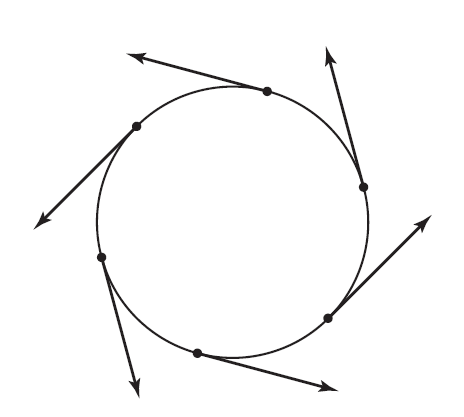
\includegraphics[scale=.6]{fig3}
	\caption{}\label{fig3}
\end{figure}

Passing to the inverse limit, as $C$ varies over all compact subsets, it follows that $U_{u}$ is itself an isomorphism. This completes the proof of 10.2. Hence we have finally completed the proof of existence (and uniqueness) for Stiefe1-Whitney classes.